% Shared preamble of the solution sheets (included by lecture01.tex, lecture02.tex, ...)
\documentclass[11pt, a4paper]{article}
\usepackage[T1]{fontenc}
\usepackage{lmodern}
\usepackage[margin=25mm]{geometry}
\usepackage{amsmath, amssymb, mathtools}
\usepackage{microtype}
\usepackage{parskip}
\usepackage{booktabs}
\usepackage{xcolor}
\usepackage{tikz}
\usetikzlibrary{patterns}
\usepackage{pgfplots}
\pgfplotsset{compat=1.18}
\usepackage{listings}
\usepackage[hidelinks]{hyperref}

% colours of the slides: Dirichlet blue, Neumann orange
\definecolor{dir}{HTML}{2A78D6}
\definecolor{neu}{HTML}{EB6834}
\definecolor{ink}{HTML}{1D2433}
\definecolor{ink2}{HTML}{52514E}
\definecolor{hair}{HTML}{C3C2B7}
\definecolor{codebg}{HTML}{F3F2EE}
\definecolor{water}{HTML}{E3EEF5}

\lstset{language=Python, basicstyle=\ttfamily\footnotesize, breaklines=true,
  postbreak=\mbox{\textcolor{ink2}{$\hookrightarrow$}\space}, keywordstyle=\color{ink}\bfseries,
  commentstyle=\color{ink2}\itshape, stringstyle=\color{ink2}, backgroundcolor=\color{codebg},
  frame=none, xleftmargin=6pt, xrightmargin=6pt, aboveskip=8pt, belowskip=8pt, columns=fullflexible,
  keepspaces=true, showstringspaces=false, upquote=true}

\setlength{\parskip}{0.6em}
\newcommand{\sheet}[2]{%
  {\small\color{ink2}\textsc{Applied math notes}}\par\vspace{-0.4em}
  {\LARGE\bfseries Lecture #1: #2}\par\vspace{0.1em}
  {\large Solutions to the exercises}\par\vspace{0.6em}}
\newcommand{\exercise}[1]{\section*{#1}}
\newcommand{\task}[1]{\par\medskip\noindent\textbf{#1}\quad}


\begin{document}
\sheet{2}{The finite element method}

%% ====================================================================== Exercise 1
\exercise{Exercise 1: Conjugate gradients and preconditioners}

\task{1.} $K = \begin{pmatrix} 3 & 2 \\ 2 & 6 \end{pmatrix}$, $F = \begin{pmatrix} 2 \\ -8 \end{pmatrix}$,
$U_0 = (-2, -2)$; the solution is $U = (2, -2)$.

\textbf{Steepest descent}, $U_{k+1} = U_k + \alpha_k\, r_k$ with $\alpha_k = r_k^T r_k / r_k^T K\, r_k$:
\[
\begin{aligned}
  r_0 &= F - K U_0 = (12, 8), & \alpha_0 &= \tfrac{208}{1200} = \tfrac{13}{75}, &
  U_1 &= \big(\tfrac{2}{25}, -\tfrac{46}{75}\big) \approx (0.080, -0.613), \\
  r_1 &= r_0 - \alpha_0 K r_0 = \tfrac{112}{75}\, (2, -3), & \alpha_1 &= \tfrac{13}{42}, &
  U_2 &= \big(\tfrac{226}{225}, -2\big) \approx (1.004, -2.000),
\end{aligned}
\]
with $K r_0 = (52, 72)$ and $K r_1 = \tfrac{112}{75}\, (0, -14)$.
The residuals are orthogonal, $r_0^T r_1 = 0$: each step turns by $90^\circ$, and after two steps the error is still
$|U - U_2| = 1.0$.

\textbf{CG} starts with the same step ($p_0 = r_0$), so $U_1$ and $r_1$ are those above. Then
\[
\begin{aligned}
  \beta_0 &= \frac{r_1^T r_1}{r_0^T r_0} = \frac{784}{5625}, &
  p_1 &= r_1 + \beta_0\, p_0 = \tfrac{1456}{5625}\, (18, -13) \approx (4.659, -3.365), \\
  \alpha_1 &= \frac{r_1^T r_1}{p_1^T K\, p_1} = \frac{75}{182}, &
  U_2 &= U_1 + \alpha_1\, p_1 = (2, -2), \qquad r_2 = 0 .
\end{aligned}
\]
CG reaches the solution after $n = 2$ steps. The directions are $K$-conjugate: $K (18, -13) = (28, -42)$ and
$p_0^T K\, p_1 \propto (12, 8) \cdot (28, -42) = 0$.

The level sets of $\Phi(U) = \tfrac12 U^T K U - U^T F$ are ellipses around $U$ with the axes along the eigenvectors of
$K$: $\lambda = 2$ for $(2, -1)$ (long axis) and $\lambda = 7$ for $(1, 2)$, condition number $3.5$. Steepest descent
(orange) zigzags, CG (blue) reaches the centre in two steps:

\begin{center}
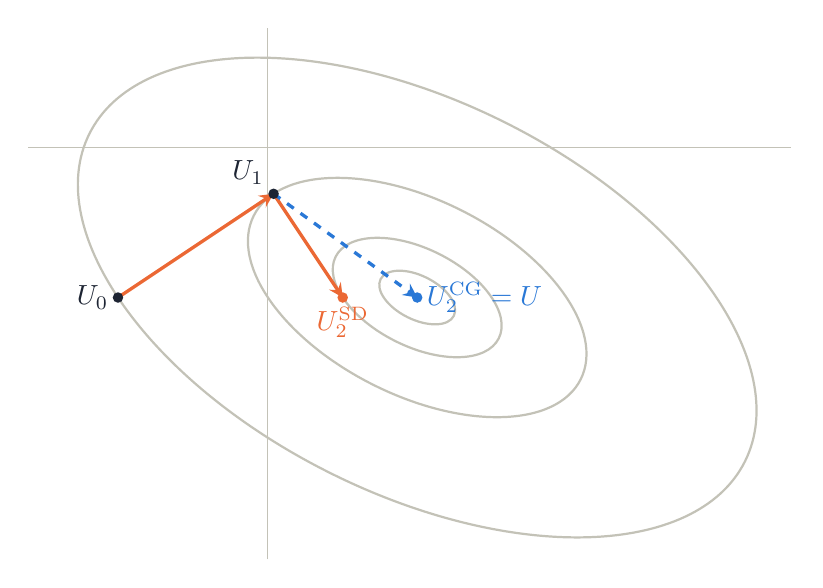
\begin{tikzpicture}[scale=0.95, >=stealth]
  \draw[hair] (-3.2, 0) -- (7.0, 0);
  \draw[hair] (0, -5.5) -- (0, 1.6);
  \foreach \c in {24, 5.973, 1.487, 0.3}
    \draw[hair, thick, rotate around={-26.565:(2, -2)}] (2, -2) ellipse ({sqrt(\c)} and {sqrt(2*\c/7)});
  \draw[neu, very thick, ->] (-2, -2) -- (0.08, -0.6133);
  \draw[neu, very thick, ->] (0.08, -0.6133) -- (1.0044, -2);
  \draw[dir, very thick, ->, dashed] (0.08, -0.6133) -- (2, -2);
  \fill[ink] (-2, -2) circle (2pt) node[left] {$U_0$};
  \fill[ink] (0.08, -0.6133) circle (2pt) node[above left] {$U_1$};
  \fill[neu] (1.0044, -2) circle (2pt) node[below, neu] {$U_2^{\mathrm{SD}}$};
  \fill[dir] (2, -2) circle (2pt) node[right, dir] {$U_2^{\mathrm{CG}} = U$};
\end{tikzpicture}
\end{center}

\task{2.} Iterations until the residual has dropped by $10^{10}$ (script below):

\begin{center}
\begin{tabular}{rrrrrr}
  \toprule
  $N$ & $n$ & none & Jacobi & ILU & AMG \\
  \midrule
    8 &     81 &    9 &    9 &   8 & 4 \\
   16 &    289 &   30 &   30 &  13 & 5 \\
   32 &   1089 &   65 &   65 &  24 & 6 \\
   64 &   4225 &  131 &  131 &  41 & 6 \\
  128 &  16641 &  264 &  264 &  76 & 6 \\
  256 &  66049 &  532 &  532 & 148 & 6 \\
  512 & 263169 & 1074 & 1074 & 292 & 6 \\
  \bottomrule
\end{tabular}
\end{center}

\begin{itemize}
  \item \textbf{Jacobi} changes nothing. On this mesh of right-angled triangles every interior row of $K$ has the
    diagonal entry $4$ (row of node 12 in example 3), so $D = 4 I$ on the coupled unknowns and $D^{-1} K = K / 4$ has
    the same condition number; CG produces the same iterates. (The Dirichlet rows are decoupled by
    \texttt{assemble\_system} and do not matter.) Jacobi helps only if the diagonal varies, e.g.\ on graded meshes
    or with varying coefficients.
  \item \textbf{ILU} needs about $3.7$ times fewer iterations, but the number still doubles with every halving of
    $h$: the condition number is reduced by a constant factor, it still grows like $h^{-2}$, and the iterations like
    $1/h = \sqrt n$ in 2D.
  \item \textbf{AMG}: the number of iterations stays constant, the work is proportional to $n$.
\end{itemize}

\lstinputlisting{lecture02_exercise1.py}

%% ====================================================================== Exercise 2
\exercise{Exercise 2: Linear elasticity, a dam}

Linear elasticity has $O(A) = 2$, $s = 1$, $m = 0$: the displacement ($c = 0$) is an essential, the traction
$\sigma n$ (first derivatives, $c = 1$) a natural boundary condition.

\task{1.}
\begin{itemize}
  \item $\Gamma_R$ (rock bed): \textcolor{dir}{\textbf{Dirichlet}}, the dam is fixed to the rock: $u = 0$.
  \item $\Gamma_W$ (water side): \textcolor{neu}{\textbf{Neumann}}, the water pressure acts against the outward normal
    and pushes the dam downstream: $\sigma n = T = -g(x)\, n$, with $n = (-1, 0)$ on the vertical face.
  \item $\Gamma_C$ (crest) and $\Gamma_A$ (air side): \textcolor{neu}{\textbf{homogeneous Neumann}}, free surfaces:
    $\sigma n = 0$.
\end{itemize}
In $g(x) = \rho\, g\, x$, $x$ is the depth below the water surface: with the vertical coordinate $y$ and the water
surface at $y = H$, $x = H - y$.

\begin{center}
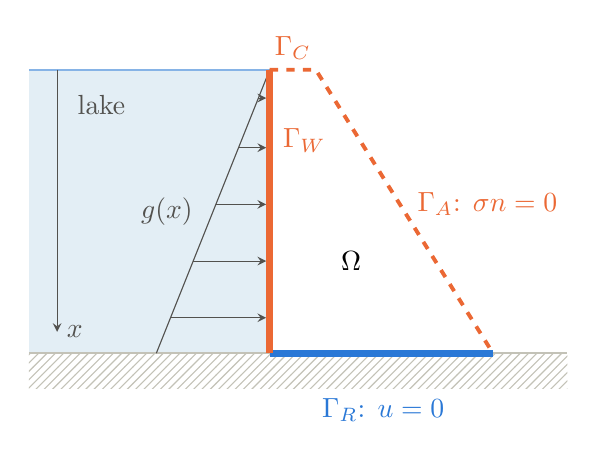
\begin{tikzpicture}[scale=0.9, >=stealth]
  \fill[water] (-3.4, 0) rectangle (0, 4);
  \draw[water!50!dir, thick] (-3.4, 4) -- (0, 4);
  \fill[pattern=north east lines, pattern color=hair] (-3.4, -0.5) rectangle (4.2, 0);
  \draw[hair, thick] (-3.4, 0) -- (4.2, 0);
  \foreach \y in {0.5, 1.3, 2.1, 2.9, 3.6}
    \draw[->, ink2] ({-1.6*(4 - \y)/4}, \y) -- (-0.05, \y);
  \draw[ink2] (0, 4) -- (-1.6, 0);
  \node[ink2, left] at (-0.95, 2.0) {$g(x)$};
  \draw[->, ink2] (-3.0, 4) -- (-3.0, 0.3) node[right] {$x$};
  \fill[white] (0, 0) -- (0, 4) -- (0.65, 4) -- (3.15, 0) -- cycle;
  \draw[dir, line width=2.4pt] (0, 0) -- (3.15, 0);
  \draw[neu, line width=2.4pt] (0, 0) -- (0, 4);
  \draw[neu, line width=1.4pt, dashed] (0, 4) -- (0.65, 4) -- (3.15, 0);
  \node at (1.15, 1.3) {$\Omega$};
  \node[neu, above] at (0.325, 4) {$\Gamma_C$};
  \node[neu, right] at (1.95, 2.1) {$\Gamma_A$: $\sigma n = 0$};
  \node[neu, right] at (0.05, 3.0) {$\Gamma_W$};
  \node[dir, below] at (1.6, -0.5) {$\Gamma_R$: $u = 0$};
  \node[ink2, left] at (-1.9, 3.5) {lake};
\end{tikzpicture}
\end{center}

\task{2.} The test functions vanish where $u$ is prescribed, $v = 0$ on $\Gamma_R$; there the traction (the unknown
reaction force of the rock) drops out of the boundary integral. On $\Gamma_W$ the traction is $T = -g(x)\, n$, on
$\Gamma_C$ and $\Gamma_A$ it is zero:
\[
  \int_{\partial\Omega} T \cdot v \; ds = -\int_{\Gamma_W} g(x)\, n \cdot v \; ds = \int_{\Gamma_W} g(x)\, v_1 \; ds .
\]
The variational form of the dam: find $u$ with $u = 0$ on $\Gamma_R$ such that
\[
  \int_\Omega \sigma(u) : \varepsilon(v) \; dx = \int_\Omega f \cdot v \; dx + \int_{\Gamma_W} g(x)\, v_1 \; ds
  \qquad \text{for all } v \text{ with } v = 0 \text{ on } \Gamma_R ,
\]
with the own weight of the concrete $f = (0, -\rho_c\, g)$ as body force ($\rho_c \approx 2400\,$kg/m$^3$, water
$\rho = 1000\,$kg/m$^3$). The essential condition on $\Gamma_R$ is built into the function space (\texttt{DirichletBC}),
the inhomogeneous natural condition on $\Gamma_W$ appears as a boundary integral, and the homogeneous ones on
$\Gamma_C$ and $\Gamma_A$ by omission.

Strong form for comparison: $-\nabla \cdot \sigma(u) = f$ in $\Omega$, $u = 0$ on $\Gamma_R$,
$\sigma n = -g(x)\, n$ on $\Gamma_W$, $\sigma n = 0$ on $\Gamma_C \cup \Gamma_A$.

\end{document}
